\documentclass{article}
\usepackage{graphicx}
\usepackage{booktabs}
\usepackage{color, colortbl}
\definecolor{Gray}{gray}{0.9}
\definecolor{LightCyan}{rgb}{0.88,1,1}
\usepackage[first=0,last=9]{lcg}

\begin{document}

    \title{Freelancing Management System \\
    \textbf{FMS}}
    \author{\textit{The Team --- Yaser, Umar, Taha and Boda}}
    \date{March 25, 2017}
\maketitle

\begin{figure}[ht!]
\centering
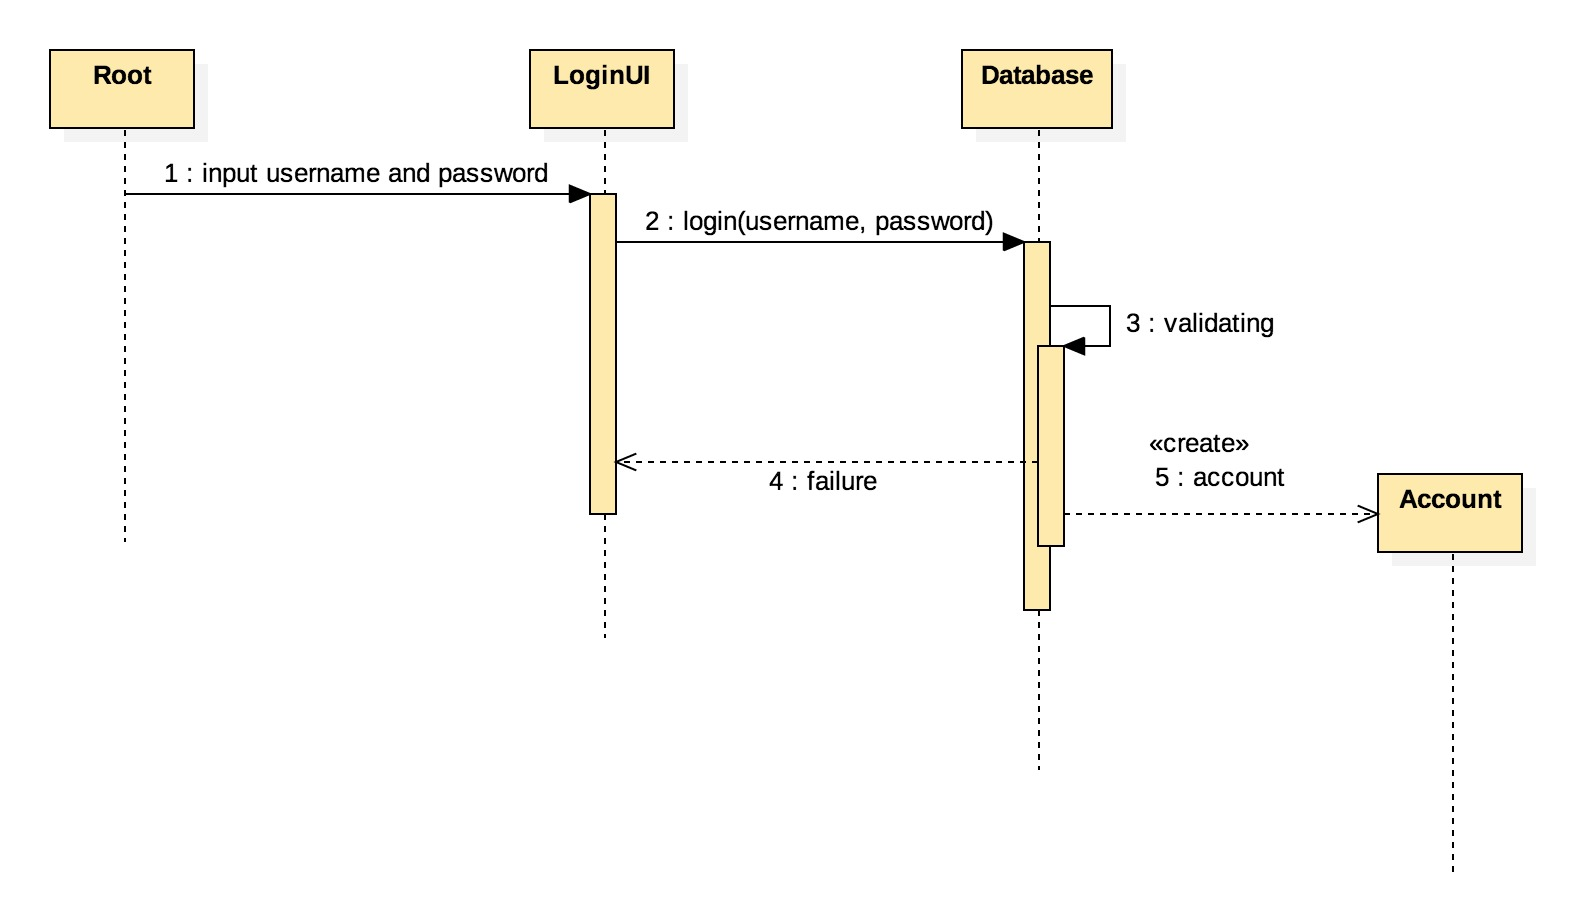
\includegraphics[width=128mm]{SequanceDiagram_Root.jpg}
\caption{System Sequence Diagram of the \textit{Root}}
\end{figure}

\newpage
\tableofcontents
\newpage



\section{System Description}
  \hspace{0.5cm} This is a \textit{Freelancing Management System}, a system which
  allows \textit{Customers } and \textit{Freelancers} to find
  one--another easily. It manages the processes from finding workers,
  verifying them, engaging, paying up to rating.
  \hspace{0.3cm}Let us take you on an interesting tour into the
  \textit{system actors}, every one of them sees the system differently
  according to their role.

\section{System Actors}
\subsection{Root}
\hspace{0.5cm} \textit{The Root} is the owner of the system. He is the one
who set it up for the first time with a special root access from him.
The Root also specifies the system settings like penalties,
bonuses on the rate and ratio of the profit on each Employer-Freelancer deal. \\
Besides, He add \textit{Admins} to manage the system.









\subsection{Admin}
\hspace{0.5cm} \textit{Admins} are the managers of the system. They have
\textit{The managers access} over the hole system, they can \textit{delete}
or \textit{ban} any consumer account. \\
Also, They can view some Statistics like the number of the Employers and
Freelancer. They can \textit{Receive} and \textit{Reply Complaints} of the
consumers as well. \\Admins can view reports about the system
 i.e \textit{economic}, \textit{consumers}, \textit{blocked}, ...   reports.

\subsection{Freelancer}
\hspace{0.5cm} \textit{Freelancers} are the workers of the system.
Every one them have an \textit{Profile} where he can share his experience,
and work examples. His \textit{Profile} contains enough information
so that the Employer can decide wherever he is going to invest in that
\textit{freelancer} or not.
There is a \textit{Rate} in the \textit{Freelancers Profile} is computed
with very accurate algorithms based on the \textit{Employers Feedback}
and how commitment is the Freelancer!
\textit{Freelancer} are paid per hour, and it is in the \textit{profile}.
A \textit{Freelancer} can review the \textit{Employers' Profiles} and
their \textit{Tasks} which they can apply for it and make special offers
for the \textit{Employers}.


\subsection{Employer}
\hspace{0.5cm} \textit{Employer} are the stockholders. They also have
their \textit{profiles}. An \textit{Employer} can create a \textit{Task} or
\textit{a list of tasks} seen  by interested \textit{Freelancers}.
Then the \textit{Employer} can choose the best \textit{Freelancer} among who
applied. Once the \textit{Employer} accepts the \textit{offer}
the money is \textit{withdrawn} from his account to the pending state in
the system. After the \textit{task} is finished, the \textit{Employer} can
\textit{rate} and \textit{feedback} the \textit{freelancer},
and sure the freelancer is paid.



\section {Diagrams}

\section{Use Case -- \textit{The Big picture}}
\begin{figure}[ht!]
\centering
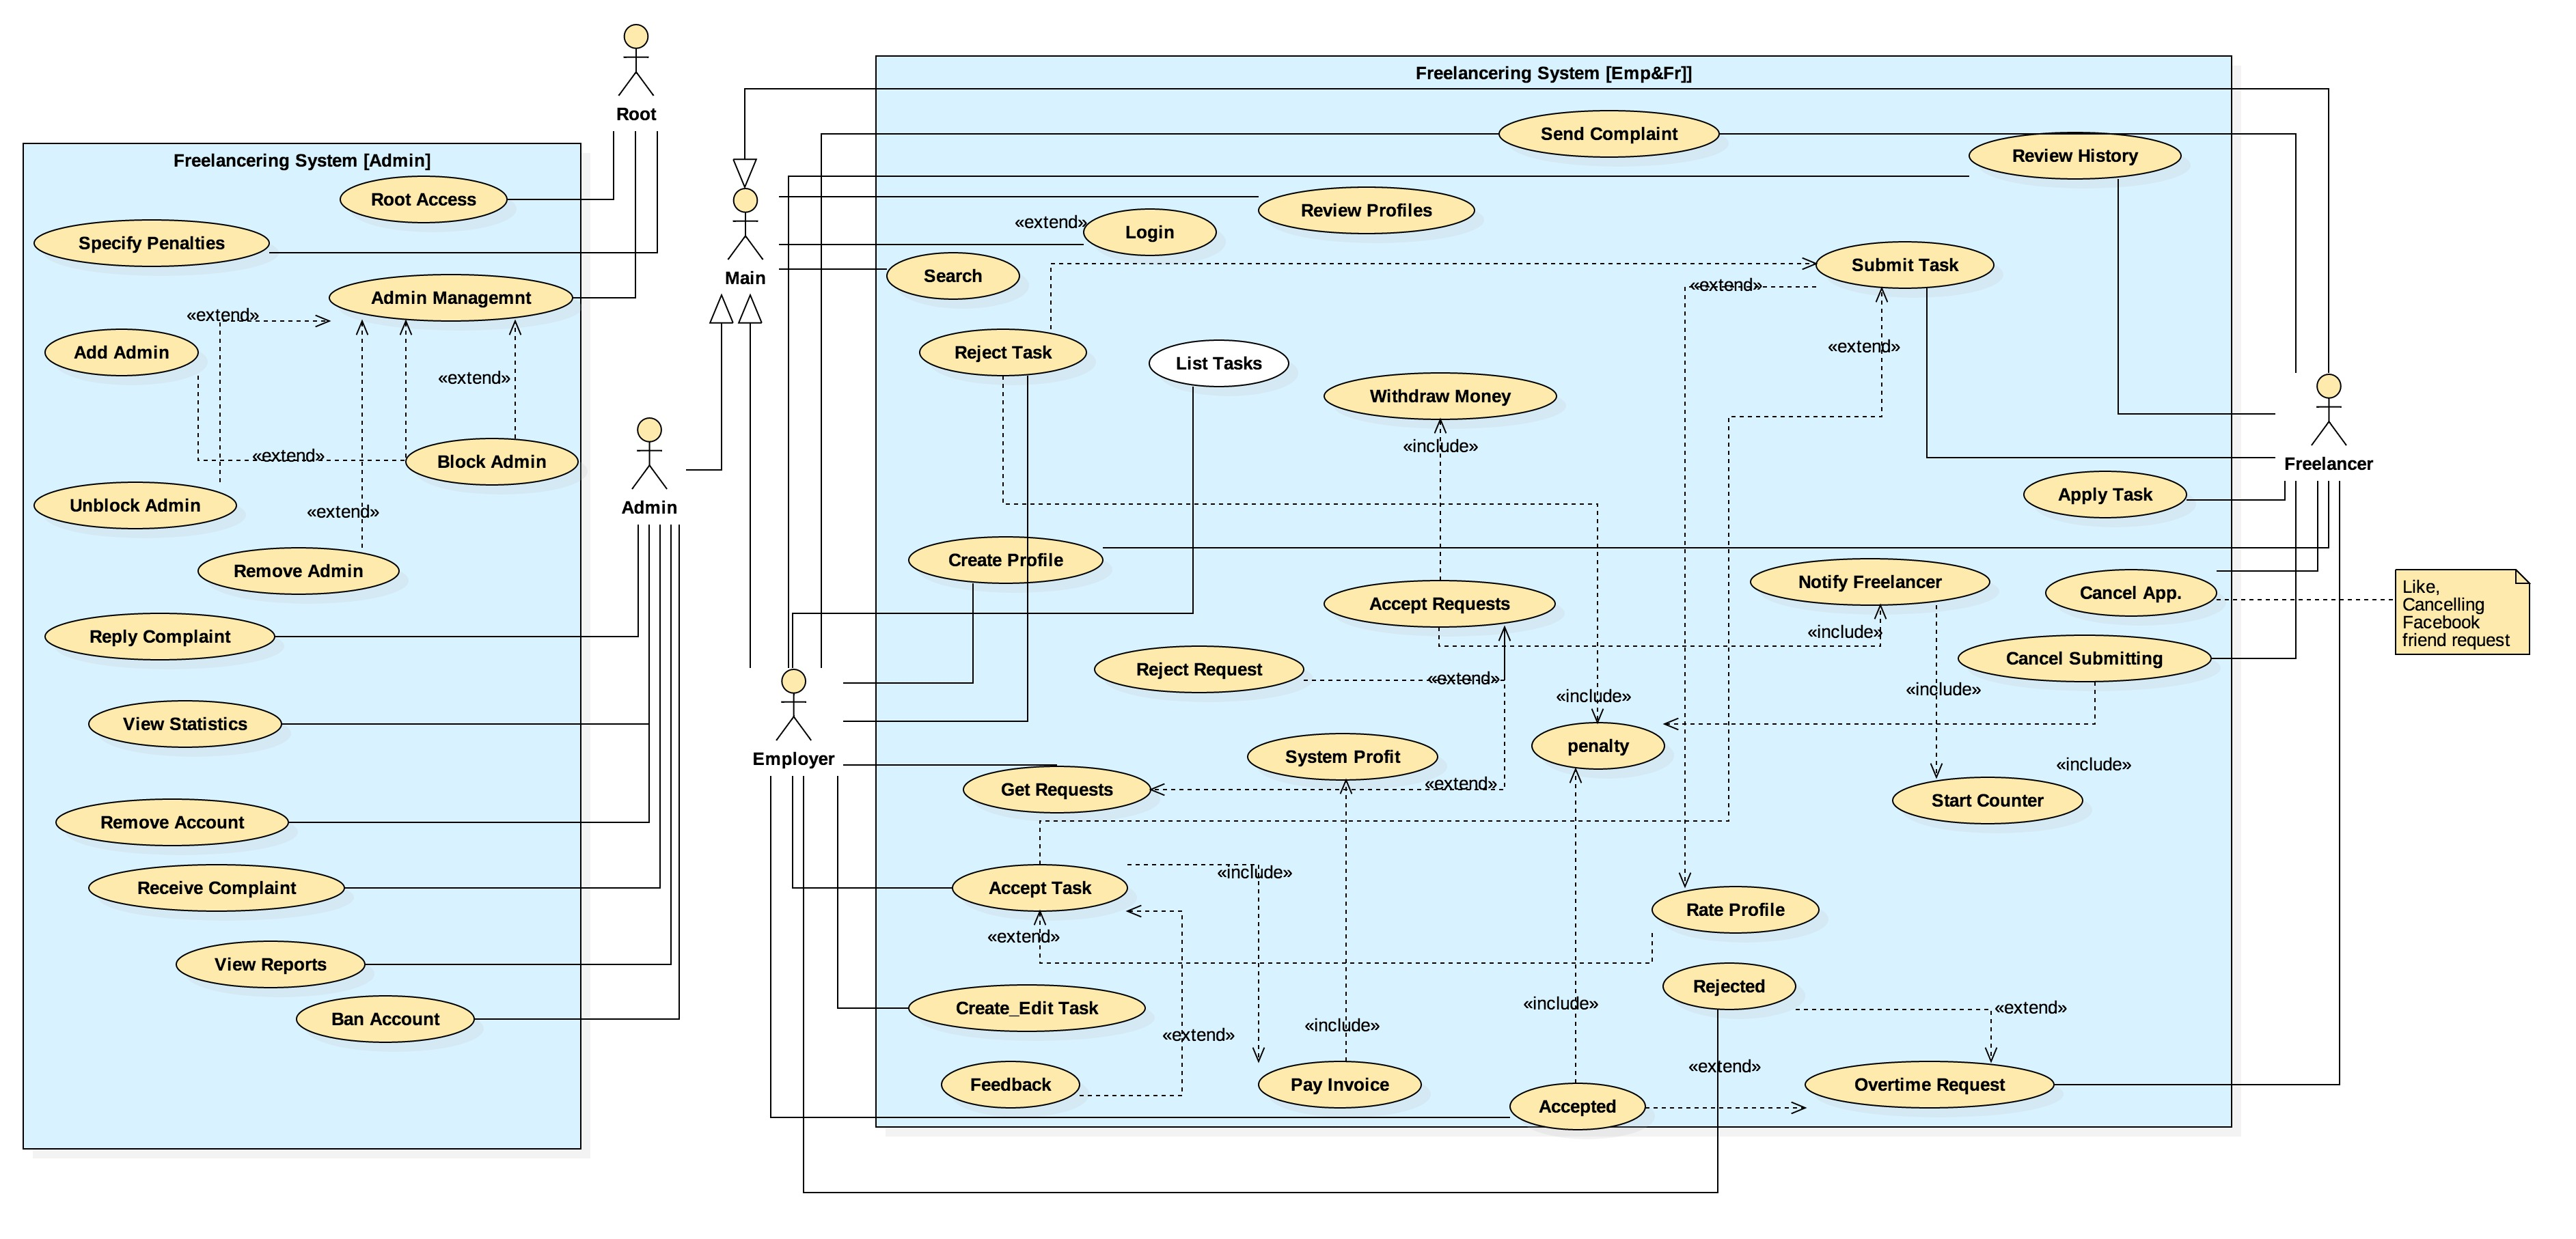
\includegraphics[width=128mm]{UseCaseDiagram_Version1}
\end{figure}


\section{Use Case -- \textit{in detail}}
\subsection{Access Root}
    \begin{tabular}{ l | l }
    \toprule
      \rowcolor{LightCyan}
      \textbf{Use Case Name}    & \textit{Root Access}\\
      \textbf{Actors}           & \textit{Root --- Exclusively}\\
      \rowcolor{LightCyan}
      \textbf{Pre--condition}   & \textit{1. At configuration time for the very first use.} \\
      \rowcolor{LightCyan}
                                & \textit{2. Root is given a default password.}\\
      \textbf{Basic Flow}       & \textit{1. Open the System}\\
                                & \textit{2. Enter `root` in the user name text box}\\
                                & \textit{3. Enter `0000` in the password text box}\\
      \rowcolor{LightCyan}
      \textbf{Post--condition}  & \textit{have full control of FMS settings}\\
    \toprule
    \end{tabular}

\subsection{Specify Penalties}
    \begin{tabular}{ l | l }
    \toprule
      \rowcolor{LightCyan}
      \textbf{Use Case Name}    & \textit{Specify Penalties}\\
      \textbf{Actors}           & \textit{Root --- Exclusively}\\
      \rowcolor{LightCyan}
      \textbf{Pre--condition}   & \textit{Root Access}\\
      \textbf{Basic Flow}       & \textit{1. Open the system with the Root Access}\\
                                & \textit{2. Click on Specifies Penalties}\\
                                & \textit{3. Fill the Data}\\
                                & \textit{4. Click submit}\\
      \rowcolor{LightCyan}
      \textbf{Post--condition}  & \textit{Penalties is configurted}\\
    \toprule
    \end{tabular}

\subsection{Add Admin}
    \begin{tabular}{ l | l }
    \toprule
      \rowcolor{LightCyan}
      \textbf{Use Case Name}    & \textit{Add Admin}\\
      \textbf{Actors}           & \textit{Root --- Exclusively}\\
      \rowcolor{LightCyan}
      \textbf{Pre--condition}   & \textit{Root Access}\\
      \textbf{Basic Flow}       & \textit{1. Open the system with the Root Access}\\
                                & \textit{2. Click Add Admin}\\
                                & \textit{3. Specify its data}\\
                                & \textit{4. Click submit}\\
      \rowcolor{LightCyan}
      \textbf{Post--condition}  & \textit{Admin is added}\\
    \toprule
    \end{tabular}



\subsection{Remove Admin}
    \begin{tabular}{ l | l }
    \toprule
      \rowcolor{LightCyan}
      \textbf{Use Case Name}    & \textit{Remove Admin}\\
      \textbf{Actors}           & \textit{Root --- Exclusively}\\
      \rowcolor{LightCyan}
      \textbf{Pre--condition}   & \textit{Root Access}\\
      \textbf{Basic Flow}       & \textit{1. Open the system with the Root Access}\\
                                & \textit{2. Click Remove Admin}\\
                                & \textit{3. Choose the Admin [drop down list}\\
                                & \textit{4. Click submit}\\
      \rowcolor{LightCyan}
      \textbf{Post--condition}  & \textit{Admin is removed}\\
    \toprule
    \end{tabular}





\subsection{Block Admin}
    \begin{tabular}{ l | l }
    \toprule
      \rowcolor{LightCyan}
      \textbf{Use Case Name}    & \textit{Block Admin}\\
      \textbf{Actors}           & \textit{Root --- Exclusively}\\
      \rowcolor{LightCyan}
      \textbf{Pre--condition}   & \textit{Root Access}\\
      \textbf{Basic Flow}       & \textit{1. Open the system with the Root Access}\\
                                & \textit{2. Click Block Admin}\\
                                & \textit{3. Choose the Admin [drop down list}\\
                                & \textit{4. Click submit}\\
      \rowcolor{LightCyan}
      \textbf{Post--condition}  & \textit{Addmin is removed and is put in the block list}\\
    \toprule
    \end{tabular}



\subsection{Unblock Admin}
    \begin{tabular}{ l | l }
    \toprule
      \rowcolor{LightCyan}
      \textbf{Use Case Name}    & \textit{Unblock Admin}\\
      \textbf{Actors}           & \textit{Root --- Exclusively}\\
      \rowcolor{LightCyan}
      \textbf{Pre--condition}   & \textit{Root Access}\\
      \textbf{Basic Flow}       & \textit{1. Open the system with the Root Access}\\
                                & \textit{2. Click Unblock Admin}\\
                                & \textit{3. Choose the Admin [drop down list}\\
                                & \textit{4. Click submit}\\
      \rowcolor{LightCyan}
      \textbf{Post--condition}  & \textit{}\\
    \toprule
    \end{tabular}


\newpage

\subsection{Search Freelancers}
    \begin{tabular}{ l | l }
    \toprule
      \rowcolor{LightCyan}
      \textbf{Use Case Name}    & \textit{Search Freelancers}\\
      \textbf{Actors}           & \textit{Employer --- Exclusively}\\
      \rowcolor{LightCyan}
      \textbf{Pre--condition}   & \textit{Employer Access}\\
      \textbf{Basic Flow}       & \textit{1. Open the system with the Employeer Access}\\
                                & \textit{2. Click Search About Freelancers}\\
                                & \textit{3. set the technologies that you want}\\
                                & \textit{4. Click submit}\\
      \rowcolor{LightCyan}
      \textbf{Post--condition}  & \textit{Show All freelancers that there Skills mathch with your Technologies}\\
    \toprule
    \end{tabular}

\begin{figure}[ht!]
\centering
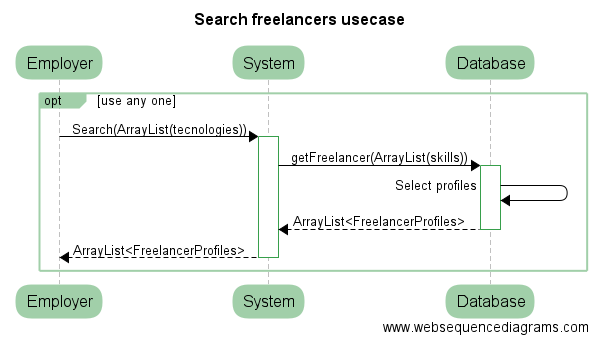
\includegraphics[width=128mm]{Search_Freelancers_usecase.png}
\end{figure}



\newpage

\subsection{Search about Freelancer}
    \begin{tabular}{ l | l }
    \toprule
      \rowcolor{LightCyan}
      \textbf{Use Case Name}    & \textit{Search about Freelancer}\\
      \textbf{Actors}           & \textit{Employer --- Exclusively}\\
      \rowcolor{LightCyan}
      \textbf{Pre--condition}   & \textit{Employer Access}\\
      \textbf{Basic Flow}       & \textit{1. Open the system with the Employer Access}\\
                                & \textit{2. Click Search About specific Freelancer}\\
                                & \textit{3. set his username or mail or phone}\\
                                & \textit{4. Click submit}\\
      \rowcolor{LightCyan}
      \textbf{Post--condition}  & \textit{Show freelancer profile}\\
    \toprule
    \end{tabular}

\begin{figure}[ht!]
\centering
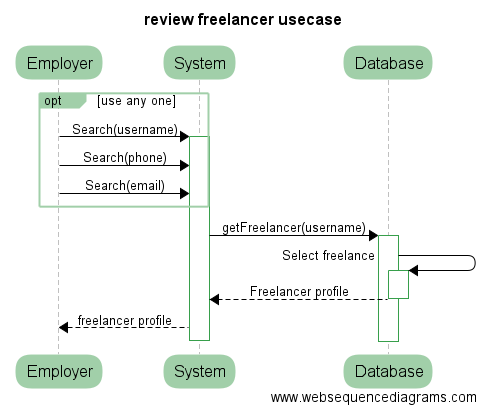
\includegraphics[width=128mm]{Search_freelancer_usecase.png}
\end{figure}


\newpage
\subsection{Review Employer history}
    \begin{tabular}{ l | l }
    \toprule
      \rowcolor{LightCyan}
      \textbf{Use Case Name}    & \textit{Review Employer history}\\
      \textbf{Actors}           & \textit{Employer --- Exclusively}\\
      \rowcolor{LightCyan}
      \textbf{Pre--condition}   & \textit{Employer Access}\\
      \textbf{Basic Flow}       & \textit{1. Open the system with the Employer Access}\\
                                & \textit{2. Click Show My history}\\
                                & \textit{3. Click submit}\\
      \rowcolor{LightCyan}
      \textbf{Post--condition}  & \textit{Show all your Tasks and offers and his modes}\\
    \toprule
    \end{tabular}

\begin{figure}[ht!]
\centering
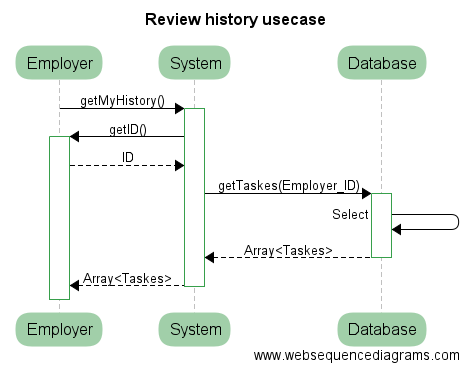
\includegraphics[width=128mm]{Review_history_usecase.png}
\end{figure}


\newpage
\subsection{Reject offer submitting }
    \begin{tabular}{ l | l }
    \toprule
      \rowcolor{LightCyan}
      \textbf{Use Case Name}    & \textit{Reject offer submitting}\\
      \textbf{Actors}           & \textit{Employer --- Exclusively}\\
      \rowcolor{LightCyan}
      \textbf{Pre--condition}   & \textit{1. Employer Access}\\
	    			& \textit{2. Task is finished but Employer need to reject it}\\
      \textbf{Basic Flow}       & \textit{1. Open the system with the Employeer Access}\\
                                & \textit{2. Check submitting Offer}\\
                                & \textit{3. Click reject this Offer}\\
      \rowcolor{LightCyan}
      \textbf{Post--condition}  & \textit{1. Take rejected}\\
	    			& \textit{2. Notify Freelancer}\\
				& \textit{3. Apply penalty}\\
    \toprule
    \end{tabular}

\begin{figure}[ht!]
\centering
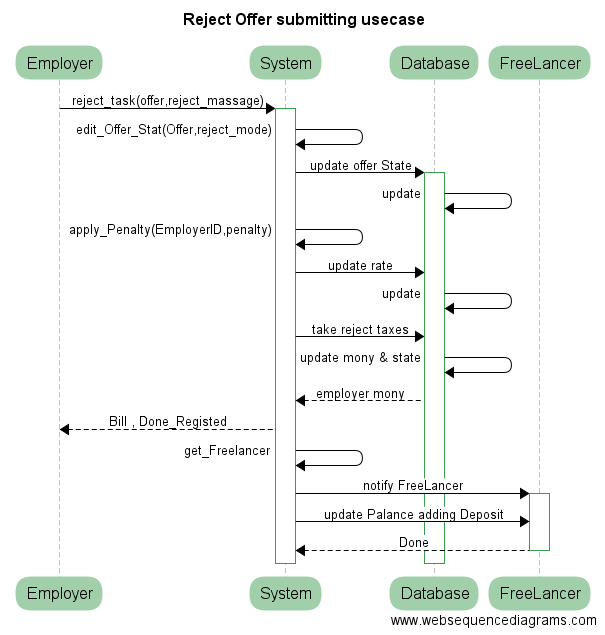
\includegraphics[width=128mm]{Reject_offer_submitting_usecase.png}
\end{figure}
\newpage

\subsection{Accept Offer}
    \begin{tabular}{ l | l }
    \toprule
      \rowcolor{LightCyan}
      \textbf{Use Case Name}    & \textit{Accept Offer}\\
      \textbf{Actors}           & \textit{Employer --- Exclusively}\\
      \rowcolor{LightCyan}
      \textbf{Pre--condition}   & \textit{1. Employer Access}\\
                                & \textit{2. Task that have offers to do it}\\
      \textbf{Basic Flow}       & \textit{1. Open the system with the Employer Access}\\
                                & \textit{2. Check Take Offer}\\
                                & \textit{3. select and Click show offer}\\
				& \textit{4. Click Accept Offer}\\

      \rowcolor{LightCyan}
      \textbf{Post--condition}  & \textit{1. change Tase mode}\\
                                & \textit{2. Notify Freelancer to start}\\
                                & \textit{3. pay deposit}\\
    \toprule
    \end{tabular}

\begin{figure}[ht!]
\centering
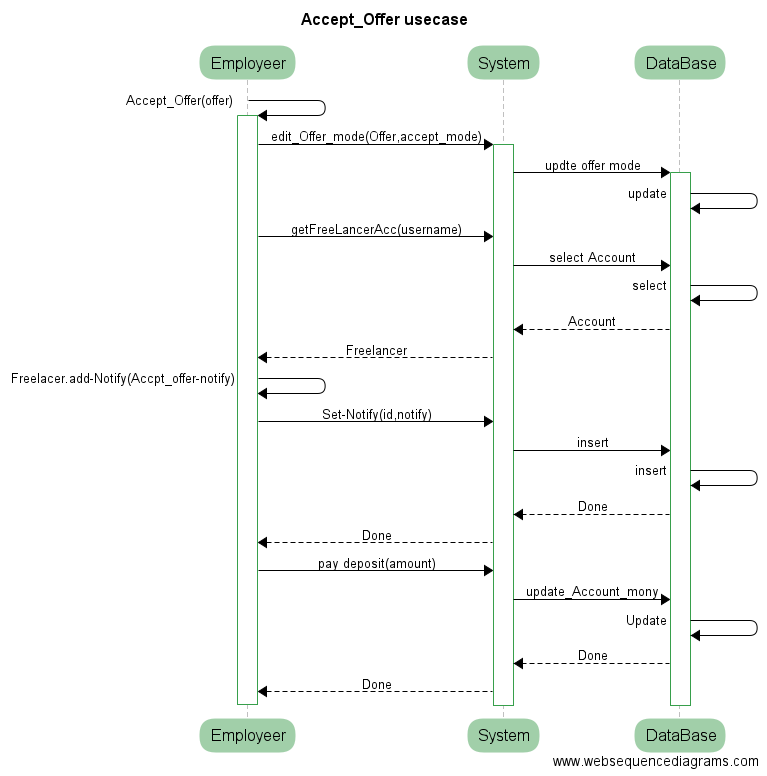
\includegraphics[width=128mm]{Accept_Offer_usecase.png}
\end{figure}

\newpage
\subsection{Accept submitting Offer}
    \begin{tabular}{ l | l }
    \toprule
      \rowcolor{LightCyan}
      \textbf{Use Case Name}    & \textit{Accept submitting Offer}\\
      \textbf{Actors}           & \textit{Employer --- Exclusively}\\
      \rowcolor{LightCyan}
      \textbf{Pre--condition}   & \textit{1. Employer Access}\\
                                & \textit{2. Task is finish and freelancer upload his work and task wait to submit from Employer}\\
      \textbf{Basic Flow}       & \textit{1. Open the system with the Employer Access}\\
                                & \textit{2. select Offer that wait submit}\\
                                & \textit{3. Click submit offer and finish task}\\
                                & \textit{4. Pay invoice}\\
				& \textit{5. Rate and FeedBack Freelancer profile}\\
      \rowcolor{LightCyan}
      \textbf{Post--condition}  & \textit{1. change account balance}\\
                                & \textit{2. re-Count to Freelancer profile}\\
                                & \textit{3. receive work}\\
    \toprule
    \end{tabular}

\begin{figure}[ht!]
\centering
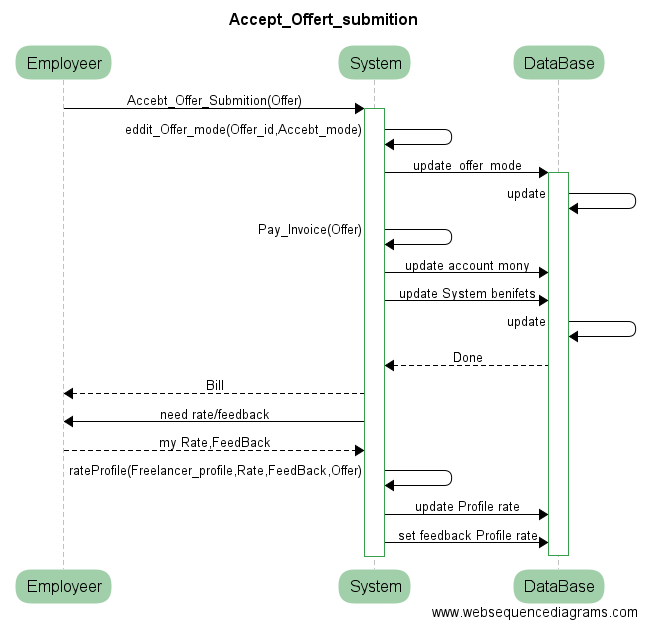
\includegraphics[width=128mm]{Accept_Offert_submition_usecase.png}
\end{figure}


\subsection{Reply Complaints}
    \begin{tabular}{ l | l }
    \toprule
      \rowcolor{LightCyan}
      \textbf{Use Case Name}    & \textit{Reply Complaints}\\
      \textbf{Actors}           & \textit{Admin}\\
      \rowcolor{LightCyan}
      \textbf{Pre--condition}   & \textit{1. Admin Access}\\
      \rowcolor{LightCyan}
                                & \textit{2. Freelancer/Employer has sent a Complaint}\\
      \textbf{Basic Flow}       & \textit{1. Open the system with the Admin Access}\\
                                & \textit{2. Select Show All Complaints from the sidebar}\\
                                & \textit{3. Select the complaint and click to reply}\\
                                & \textit{4. Write your reply and submit}\\
      \rowcolor{LightCyan}
      \textbf{Post--condition}  & \textit{A notification has sent to the sender of the commitment}\\
    \toprule
    \end{tabular}


\subsection{View Statistics}
    \begin{tabular}{ l | l }
    \toprule
      \rowcolor{LightCyan}
      \textbf{Use Case Name}    & \textit{View Statistics}\\
      \textbf{Actors}           & \textit{Admin}\\
      \rowcolor{LightCyan}
      \textbf{Pre--condition}   & \textit{1. Admin Access}\\
                                  \rowcolor{LightCyan}
                                & \textit{2. Freelancer/Employer has sent a Complaint}\\
      \textbf{Basic Flow}       & \textit{1. Open the system with the Admin Access}\\
                                & \textit{2. Select View Statistics from the sidebar}\\
                                & \textit{3. Now, You can select one of the statistics perspective}\\
      \rowcolor{LightCyan}
      \textbf{Post--condition}  & \textit{A graph is appeared}\\
    \toprule
    \end{tabular}




\subsection{Remove Account}
    \begin{tabular}{ l | l }
    \toprule
      \rowcolor{LightCyan}
      \textbf{Use Case Name}    & \textit{Remove Account}\\
      \textbf{Actors}           & \textit{Admin}\\
      \rowcolor{LightCyan}
      \textbf{Pre--condition}   & \textit{1. Admin Access}\\
                                  \rowcolor{LightCyan}
                                & \textit{2. Freelancer/Employer has sent a Complaint}\\
      \textbf{Basic Flow}       & \textit{1. Open the system with the Admin Access}\\
                                & \textit{2. Select Show All Freelancer/Employer from the sidebar}\\
                                & \textit{3. Select the one you want to removed}\\
                                & \textit{4. Select Remove Account}\\
                                & \textit{5. Confirm!}\\
      \rowcolor{LightCyan}
      \textbf{Post--condition}  & \textit{An Account it removed}\\
    \toprule
    \end{tabular}




\subsection{Receive Complaint}
    \begin{tabular}{ l | l }
    \toprule
      \rowcolor{LightCyan}
      \textbf{Use Case Name}    & \textit{Receive Complaint}\\
      \textbf{Actors}           & \textit{Admin}\\
      \rowcolor{LightCyan}
      \textbf{Pre--condition}   & \textit{1. Admin Access}\\
                                  \rowcolor{LightCyan}
                                & \textit{2. Freelancer/Employer has sent a Complaint}\\
      \textbf{Basic Flow}       & \textit{1. Open the system with the Admin Access}\\
                                & \textit{2. You will find a new notification}\\
      \rowcolor{LightCyan}
      \textbf{Post--condition}  & \textit{You've been notified}\\
    \toprule
    \end{tabular}




\subsection{View Reports}
    \begin{tabular}{ l | l }
    \toprule
      \rowcolor{LightCyan}
      \textbf{Use Case Name}    & \textit{View Reports}\\
      \textbf{Actors}           & \textit{Admin}\\
      \rowcolor{LightCyan}
      \textbf{Pre--condition}   & \textit{1. Admin Access}\\
                                  \rowcolor{LightCyan}
                                & \textit{2. Freelancer/Employer has sent a Complaint}\\
      \textbf{Basic Flow}       & \textit{1. Open the system with the Admin Access}\\
                                & \textit{2. Select View Reports}\\
                                & \textit{3. Select the Subject of the Report}\\
      \rowcolor{LightCyan}
      \textbf{Post--condition}  & \textit{You have an up-to-date report, you can get the PDF version}\\
    \toprule
    \end{tabular}





\subsection{Ban Account}
    \begin{tabular}{ l | l }
    \toprule
      \rowcolor{LightCyan}
      \textbf{Use Case Name}    & \textit{Ban Account}\\
      \textbf{Actors}           & \textit{Admin}\\
      \rowcolor{LightCyan}
      \textbf{Pre--condition}   & \textit{1. Admin Access}\\
                                  \rowcolor{LightCyan}
                                & \textit{2. Freelancer/Employer has sent a Complaint}\\
      \textbf{Basic Flow}       & \textit{1. Open the system with the Admin Access}\\
                                & \textit{2. Select Show All Freelancer/Employer from the sidebar}\\
                                & \textit{3. Select the one you want to Ban}\\
                                & \textit{4. Select Ban Account}\\
                                & \textit{4. Confirm!}\\
      \rowcolor{LightCyan}
      \textbf{Post--condition}  & \textit{An Account is Banned}\\
    \toprule
    \end{tabular}






\newpage


\section{Design Patterns}

\subsection{Singleton Design Pattern}
    \begin{tabular}{ l | l }
    \toprule
      \rowcolor{LightCyan}
      \textbf{Context}            & \textit{}\\
      \textbf{Problem}            & \textit{}\\
                                  & \textit{}\\
      \rowcolor{LightCyan}
      \textbf{Solution}           & \textit{}\\
      \textbf{Post--condition}    & \textit{}\\
                                  & \textit{}\\
                                  & \textit{}\\
    \toprule
    \end{tabular}

\begin{figure}[ht!]
\centering
%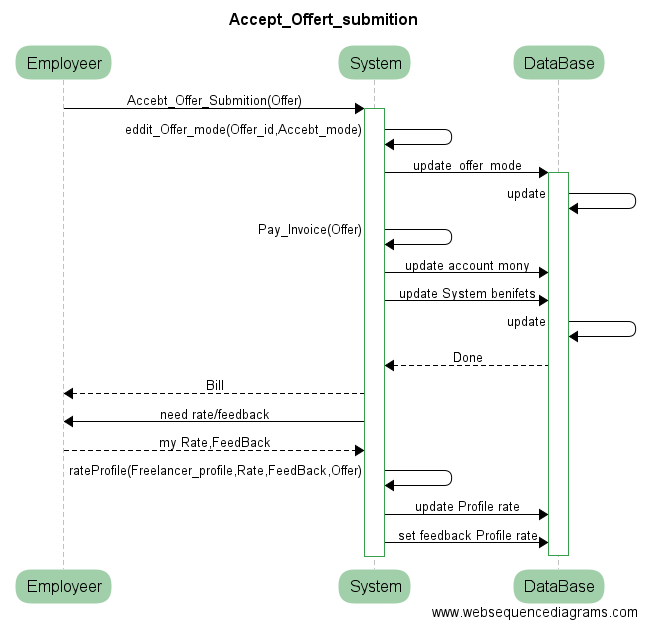
\includegraphics[width=128mm]{Accept_Offert_submition_usecase.png}
\end{figure}






\section{Call Us}







\end{document}
